%*******************************************************************************
%****************************** Second Chapter *********************************
%*******************************************************************************

\chapter{Thiết kế và hiện thực \newline sản phẩm móc khóa thông minh - Smart Keyring}

\ifpdf
    \graphicspath{{Chapter2/Figs/Raster/}{Chapter2/Figs/PDF/}{Chapter2/Figs/}}
\else
    \graphicspath{{Chapter2/Figs/Vector/}{Chapter2/Figs/}}
\fi


%\section[Short title]{Reasonably long section title}
\section{Thiết kế sản phẩm}
% Uncomment this line, when you have siunitx package loaded.
%The SI Units for dynamic viscosity is \si{\newton\second\per\metre\squared}.
\textit{Thiết kế tính năng sản phẩm:}

\label{feature}
Sản phẩm Smart Keyring sẽ có các tính năng cơ bản như:

• Báo hiệu khi mất kết nối: hỗ trợ việc cảnh báo người tránh bỏ quên 1 trong 2 thiết bị.

• Báo hiệu khi kích hoạt chức năng tìm kiếm: cho phép người dùng định vị thiết bị còn lại trong phạm vi kết nối.

• Hai chế độ báo hiệu bằng âm thanh hoặc ánh sáng đèn led hoặc cả 2: mục đích sử dụng trong nhiều trường hợp khác nhau như đêm tối, không gian yên tĩnh...
\section{Các hướng tiếp cận vấn đề}

Tại thời điểm tìm hiểu và hiện thực đề tài NCKH, tại Việt Nam chỉ có module HM-10 có sử dụng chip BLE CC2540/2541 được phát triển thành board mạch hoàn chỉnh nên phần này chỉ nói về hướng phát triển với board mạch này.

\begin{figure}[h]
	\centering    
	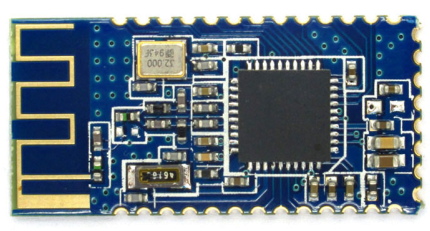
\includegraphics[width=1.0\textwidth]{hm10}
	\caption[Module BLE HM-10]{Module BLE HM-10}
	\label{fig: c2-hm10}
\end{figure}

\subsection{Phát triển thiết bị chỉ dựa vào SoC CC2540/2541}

Về hướng này chúng ta sẽ phát triển lập trình thiết bị chỉ trên duy nhất 1 SoC CC2540/2541.

\textbf{Ưu điểm}: 

• Có thể thu nhỏ thiết kế đến mức tối thiểu

• Viết ứng dụng ngay trên nền tảng BLE sẽ tiết kiệm tối đa năng lượng tiêu thụ.

\textbf{Nhược điểm}: 

• Bị hạn chế về khả năng phát triển cả về phần cứng lẫn phần mềm.

• Không tìm được source code firmware cho module.

• Không có tài liệu chính thống nào hướng dẫn các bước lập trình cho vi điều khiển CC2540/2541 được tích hợp trên module HM-10

• Nhà sản xuất không công khai thiết kế mạch của sản phẩm HM-10

• Chỉ có duy nhất 1 phần mềm hỗ trợ các gói thư viện lập trình cho CC2540/2541 là IAR Embedded Workbench for 8051 thuộc Texas Instrument nhưng bản quyền cho phần mềm có giá quá cao và các thư viện này sử dụng mã nguồn đóng nên không chuyển sang các phần mềm khác được.

\textit{Vì những cản trở đó, nhóm quyết định chuyển sang phương pháp tiếp cận khác đơn giản và khả thi hơn.}

\subsection{Kết hợp MCU và Module BLE HM-10}
Cách tiếp cận này khá quen thuộc với đa số hệ thống và sản phẩm hiện nay bao gồm 1 vi điều khiển trung tâm: chứa toàn bộ chương trình hoạt động của sản phẩm và các thiết bị ngoại vi (sensor, các module giao tiếp rf, Bluetooth…)

\textbf{Ưu điểm: }

• Dễ tiếp cận, do người hiện thực có thể kiểm soát được công nghệ mình sử dụng

• Tùy biến các loại vi điều khiển sao cho thích hợp nhất đối với yêu cầu đề tài. Các vi điều khiển riêng rẻ hiện nay rất đa dạng chủng loại và chức năng, đi kèm theo nó là hệ thống hỗ trợ cực kì tốt từ nhà sản xuất về tài liệu, môi trường lập trình, các forum trao đổi. điển hình là các thương hiệu Atmel, Microchip…

\textbf{Nhược điểm:} 

• Đối nghịch lại với ưu điểm của cách tiếp cận đầu tiên thì hướng tiếp cận này sẽ cần nhiều không gian hơn (thêm 1 vi điều khiển).

• Làm cho hệ thống mất đi tính linh động và gọn nhẹ so với tính chất sản phẩm cũng như là năng lượng tiêu thụ không được tối ưu.

• Thêm 1 vi điều khiển tương đương với việc thêm 1 nguồn tiêu thụ điện, giảm thời gian hoạt động của sản phẩm.

\section{Sơ đồ hoạt động}
\subsection{Tổng quát}
Sơ đồ hoạt động tổng quát:

\begin{figure}[h]
	\centering    
	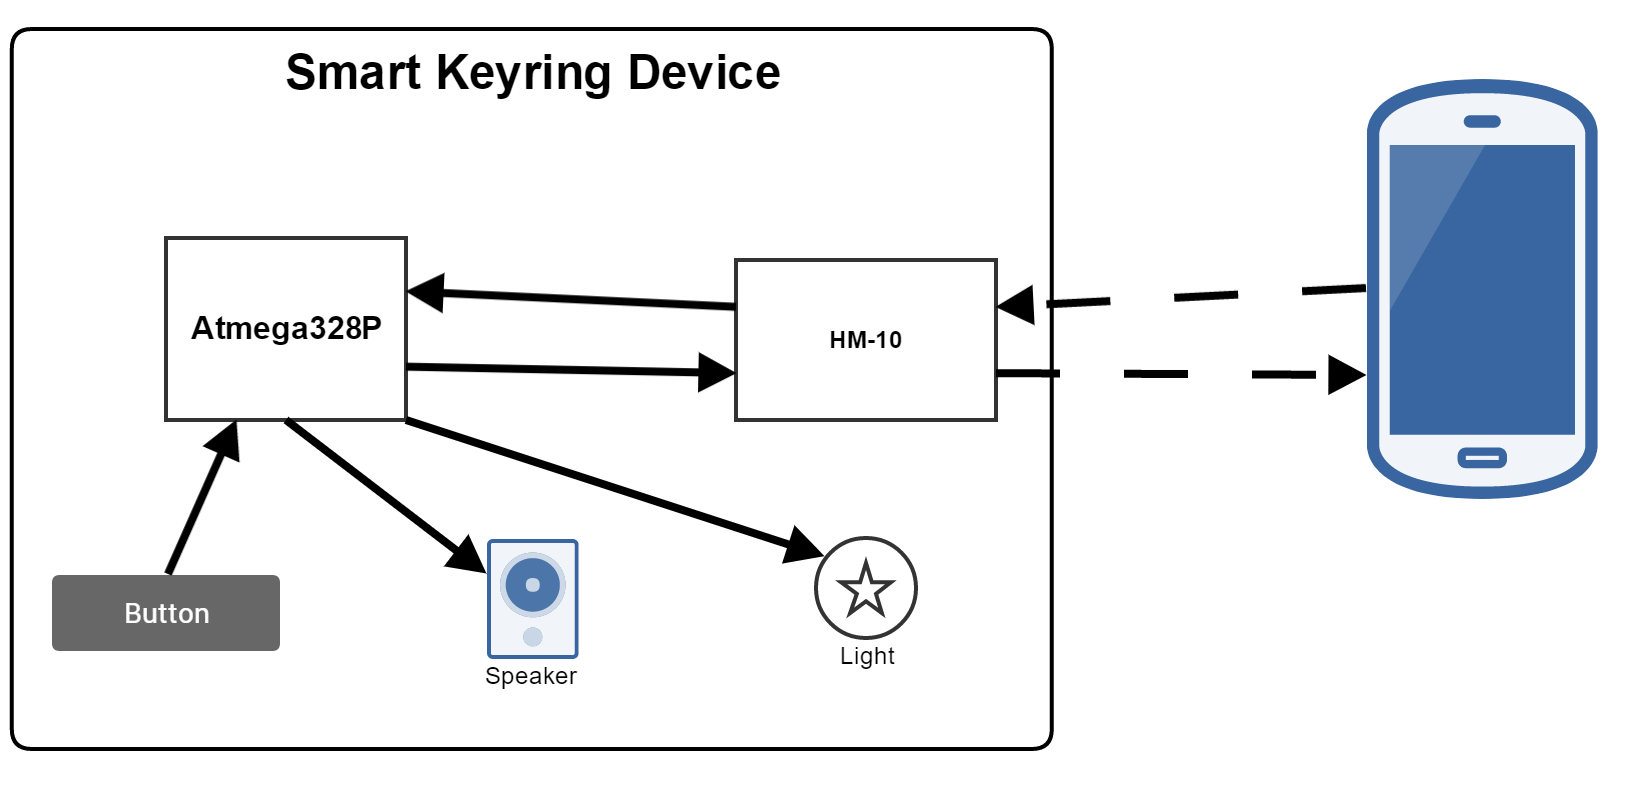
\includegraphics[width=1.0\textwidth]{general}
	\caption[Sơ đồ hoạt động tổng quát]{Sơ đồ hoạt động tổng quát}
	\label{fig: general}
\end{figure}

Như hình \ref{fig: general}, thiết bị Smart Keyring giao tiếp với thiết bị di động thông qua module BLE HM-10 và được điều khiển bởi MCU ATmega328P đảm nhận chức năng quản lý I/O như nút ấn, loa báo hiệu và đèn cũng như là truyền nhận thông điệp với module HM10.

\subsection{Nhận lệnh báo từ thiết bị di động}

Chức năng tìm kiếm thiết bị được kích hoạt bởi thiết bị di động được mô tả ở hình \ref{fig: ring1}.

Trình tự các hoạt động như sau:

(1) Thiết bị di động gửi gói tin với nội dung yêu cầu phát tín hiệu báo tới module HM-10.

(2) MCU ATmega328P nhận gói tin từ module HM-10 bằng giao thức UART với chế độ interrupt.

(3) Loa và đèn báo hiệu được kích hoạt tùy theo nội dung gói tin: kích hoạt cả hai hoặc chỉ kích hoạt đèn báo hiệu

(4*) Nút nhấn có chức năng ngắt chế độ báo hiệu khi cần thiết thông qua interrupt GPIO

\begin{figure}[h]
	\centering    
	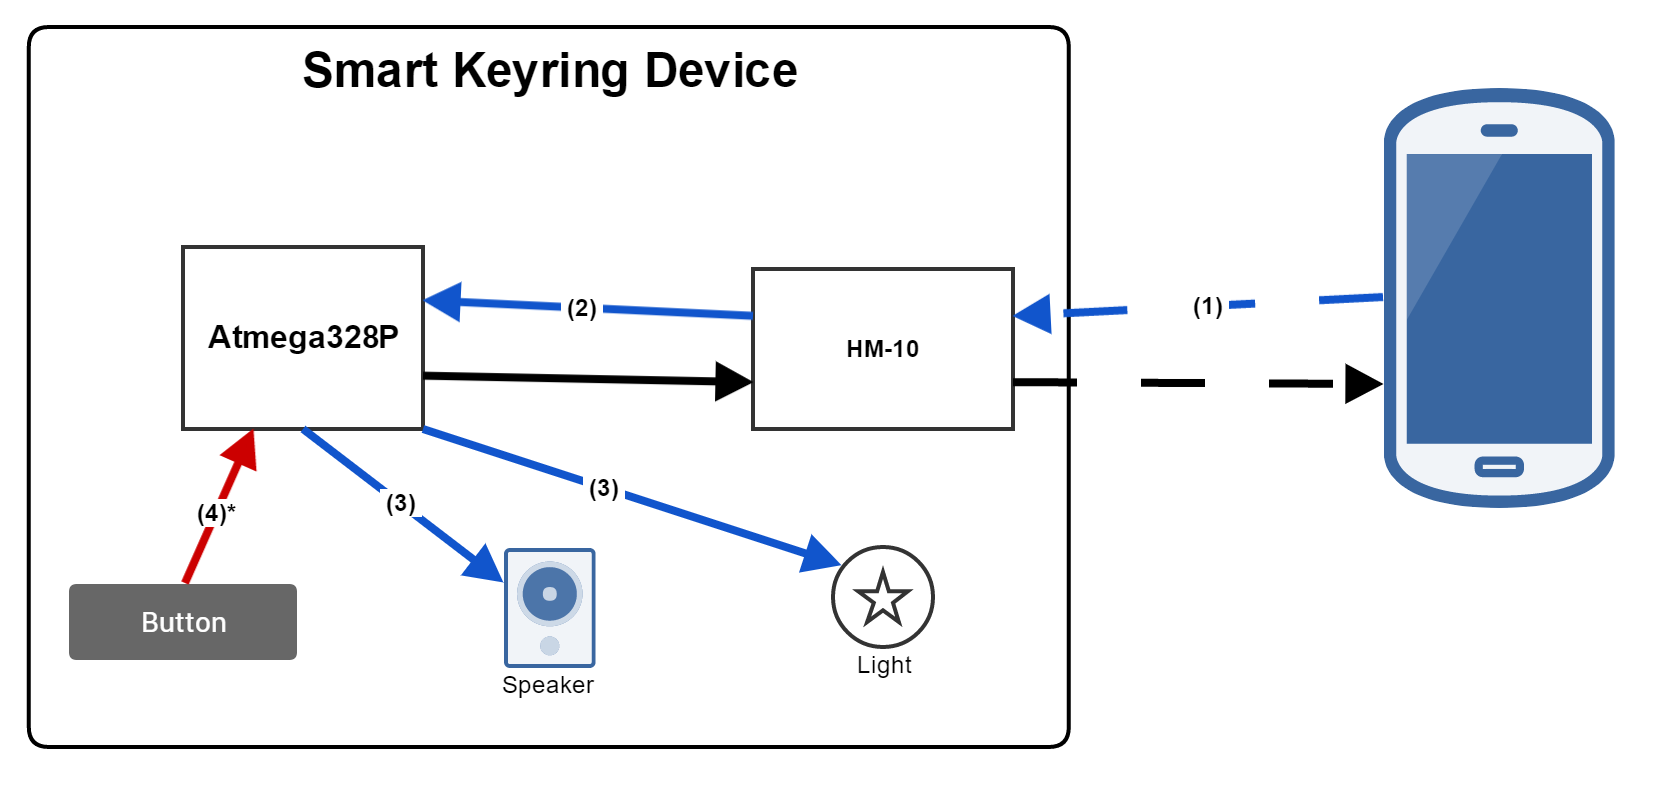
\includegraphics[width=1.0\textwidth]{ring1}
	\caption[Sơ đồ hoạt động khi nhận lệnh báo từ thiết bị di động]{Sơ đồ hoạt động khi nhận lệnh báo từ thiết bị di động}
	\label{fig: ring1}
\end{figure}

Sơ đồ hoạt động trên đúng với chức năng ngắt báo hiệu thiết bị được điều khiển bởi thiết bị di động, chỉ khác tại bước (3) là ngắt loa và đèn và không có bước (4).
\subsection{Kích hoạt thiết bị di động bật chế độ báo hiệu}

Chức năng kích hoạt thiết bị di động bật chế độ báo hiệu được mô tả ở hình \ref{fig: ring2}.

Trình từ các hoạt động như sau:

(1) MCU ATmega328P nhận tín hiệu điều khiển từ nút ấn thông qua interrupt GPIO

(2) Module BLE HM-10 nhận gói tin điều khiển từ MCU ATmega328 thông qua UART

(3) Thiết bị di động nhận gói tin truyền từ Module HM-10 và kích hoạt chế độ báo hiệu

\begin{figure}[h]
	\centering    
	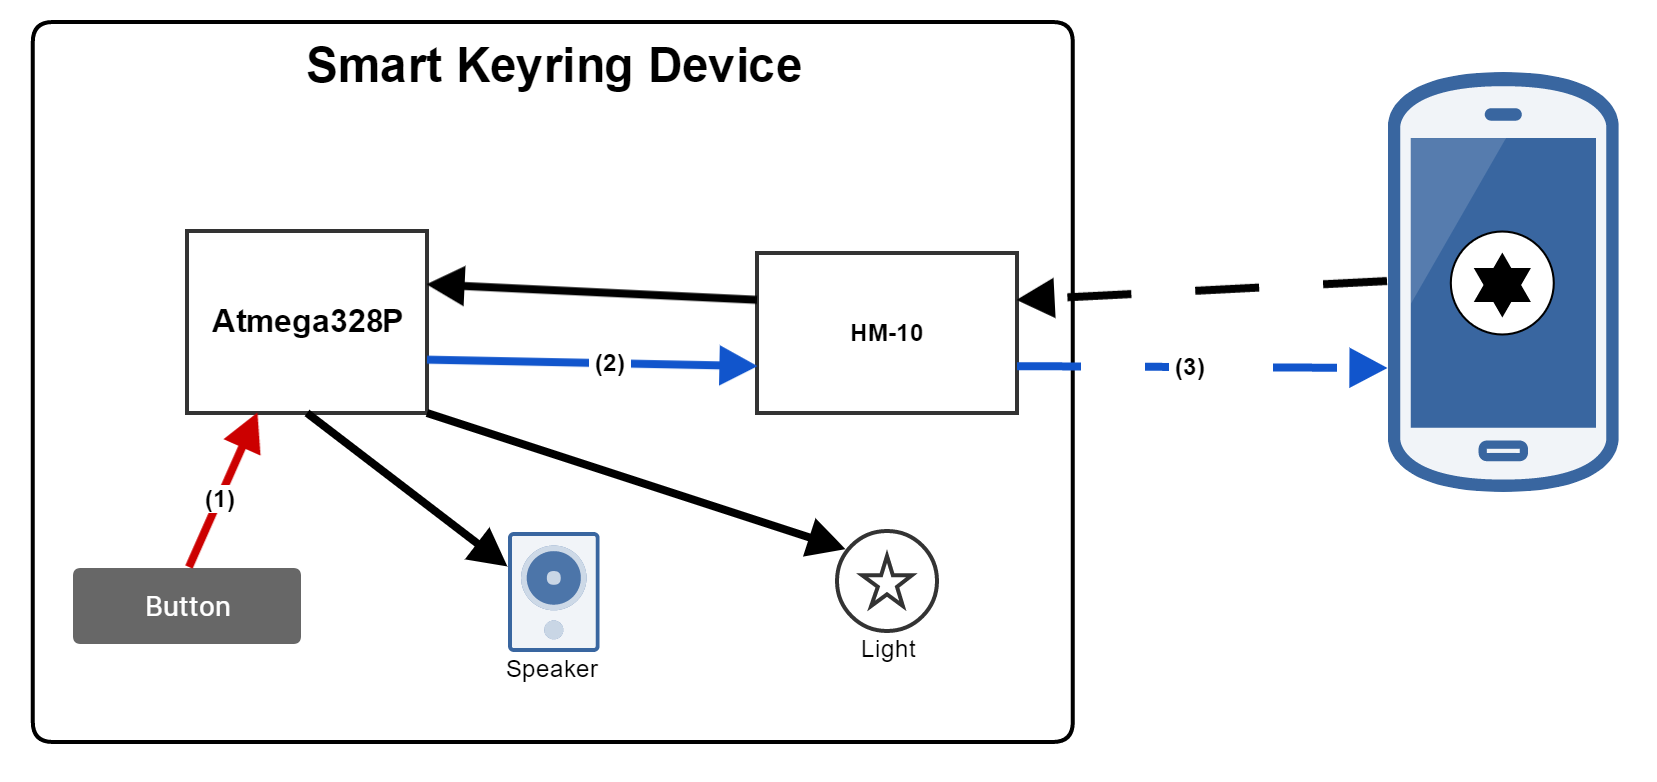
\includegraphics[width=1.0\textwidth]{ring2}
	\caption[Sơ đồ kích hoạt thiết bị di động bật chế độ báo hiệu]{Sơ đồ kích hoạt thiết bị di động bật chế độ báo hiệu}
	\label{fig: ring2}
\end{figure}
\newpage

\subsection{Sơ đồ trạng thái hoạt động khi ngắt kết nối}
Dựa theo tính năng sản phẩm ở mục \ref{feature}, sơ đồ trạng thái hoạt động được thiết kế ở hình \ref{fig: ble} và \ref{fig: blelost}

	\begin{figure}[h]
		\centering    
		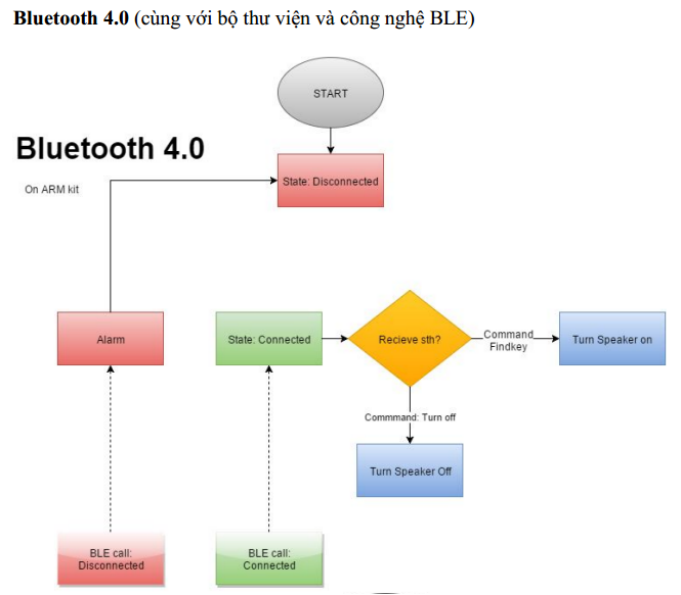
\includegraphics[width=1.0\textwidth]{ble}
		\caption[Sơ đồ trạng thái trên thiết bị Smart Keyring]{Sơ đồ trạng thái trên thiết bị Smart Keyring}
		\label{fig: ble}
	\end{figure}
	
	\begin{figure}[h]
		\centering    
		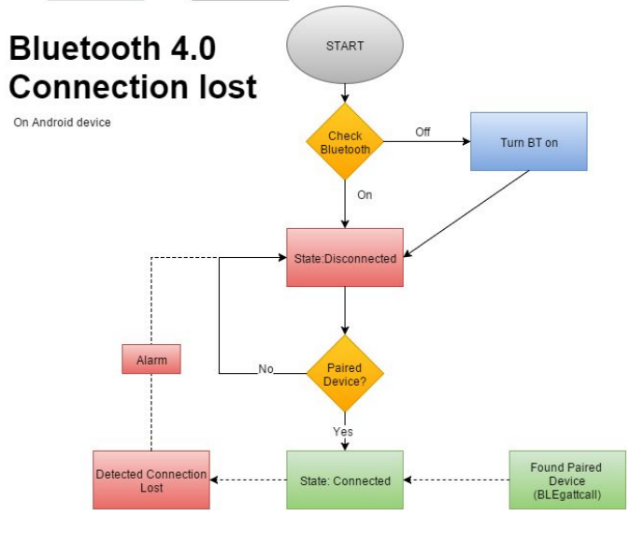
\includegraphics[width=1.0\textwidth]{blelost}
		\caption[Sơ đồ hoạt động trên thiết bị di động]{Sơ đồ hoạt động trên thiết bị di động}
		\label{fig: blelost}
	\end{figure}
\newpage
\section{Hiện thực phần cứng}
\subsection{Thiết kế board mạch}
Theo như yêu cầu chức năng ở mục \ref{feature}, schematic được thiết kế như hình \ref{fig: schematic}

Các thiết bị linh kiện bao gồm:

• 01 MCU ATmega328P

• 01 Module BLE HM-10

• 01 LED báo hiệu

• 01 Buzzer

• 01 Nút bấm

• Các tụ và trở bổ sung

	\begin{figure}[!ht]
		\centering    
		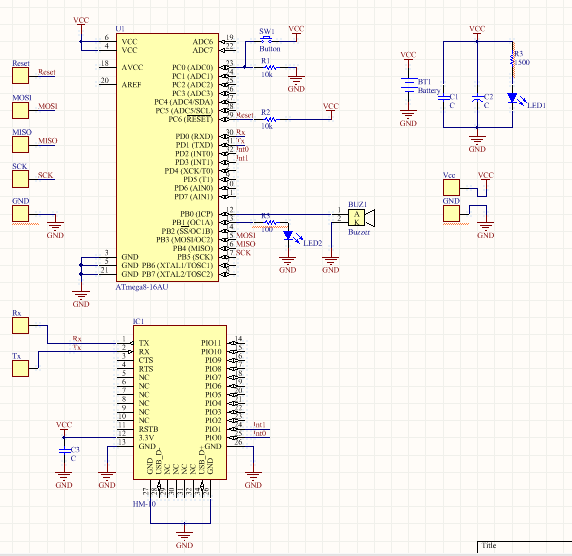
\includegraphics[width=1.0\textwidth]{schematic}
		\caption[Schematic của thiết bị Smart Keyring]{Schematic của thiết bị Smart Keyring}
		\label{fig: schematic}
	\end{figure}
	
\subsection{Hiện thực thiết bị}



\section{Hiện thực ứng dụng di động trên Android}

\subsection{Các khái niệm trong lập trình BLE trên Android}
%TODO: https://developer.android.com/guide/topics/connectivity/bluetooth-le.html
Dưới đây là những khái niệm chính về BLE được sử dụng:

\textbf{Generic Attribute Profile (GATT) -  Cấu hình thuộc tính chung }— Cấu hình GATT là đặc điểm kỹ thuật chung cho việc truyền nhận các gói dữ liệu nhỏ được biết đến như là các "đặc tính" trên đường truyền BLE. Tất cả các cấu hình ứng dụng BLE đều dựa trên GATT.

\textbf{Attribute Protocol (ATT) - Thuộc tính của giao thức}—GATT được xây dựng bên trên lớp ATT, thường được nhắc đến là GATT/ATT. ATT được tối ưu hóa trên các thiết bị BLE và sử dụng ít dữ liệu nhất có thể. Các thuộc tính này được định danh duy nhất bởi Universally Unique Identifier (UUID), là 1 chuỗi định danh dưới chuẩn 128-bit để định danh thông tin duy nhất. Các thuộc tính được truyền bởi ATT được định dạng dưới các characteristics và services.

\textbf{Characteristic}—A characteristic contains a single value and 0-n descriptors that describe the characteristic's value. A characteristic can be thought of as a type, analogous to a class. 

\textbf{Descriptor}—Descriptors are defined attributes that describe a characteristic value. For example, a descriptor might specify a human-readable description, an acceptable range for a characteristic's value, or a unit of measure that is specific to a characteristic's value.

\textbf{Service}— Service là một gói tổng hợp các characteristic. Ví dụ, ta có thể có service gọi là "Theo dõi nhịp tim" vừa bao gồm các characteristic như "đo nhịp tim". Danh sách các cấu hình GATT và service có thể tìm thấy tại bluetooth.org

\subsection{Phát triển ứng dụng Android}
